\subsection*{EAN-13 Code}
\writtenby{\dcauthornameriren}%
% normale
Strichcodes sind sich im Allgemeinen sehr ähnlich und unterscheiden sich maximal durch die Strichbreite und -länge. Die Länge ist allerdings für die aktuelle Unter\-suchung nicht von Interesse, denn diese bietet maximal eine leichte Fehlertoleranz, aber keinen Unterschied in der Erkennungsleistung. Die Strichbreite dagegen ermöglicht eine höhere Robustheit in der Erkennung. Daher untersuchen wir, wie in Abbild\-ung \ref{fig:eannormal} Bild 1 und 2 zu sehen ist, nur 2 unterschiedliche Strichstärken. 

Strichcodes besitzen keine große Fehlertoleranz, wie z.B. QR-Codes, aber sie besitz\-en trotzdem einen großen Vorteil, nämlich dass eine gute Scanline für die Erkennung ausreicht, wie z.B. in Abbildung \ref{fig:eannormal} Bild 3.
\begin{figure}[H]
  \centering
  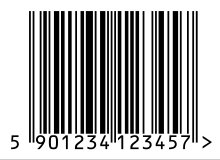
\includegraphics[width=0.30\textwidth]{img/EAN13/perfect_01.jpg}
  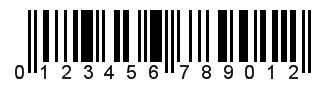
\includegraphics[width=0.35\textwidth]{img/EAN13/perfect_02.jpg}
  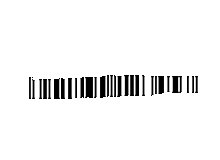
\includegraphics[width=0.30\textwidth]{img/EAN13/compensation_01.jpg}
  \caption{EAN-13 normale Größe, klein, partieller Code}
  \label{fig:eannormal}
\end{figure}

% unscharfe
Bei unscharfen Bildern macht sich die Strichbreite sofort bemerkbar, denn für die normale Breite ist bereits eine leichte Unschärfe~(Abbildung \ref{fig:eanblurry} Bild 1) inakzeptabel. Bei den breiteren Strichen allerdings ist selbst bei einer mehr als 4 mal so hohen Unschärfe noch eine Dekodierung möglich.
\begin{figure}[H]
  \centering
  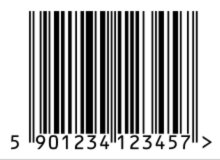
\includegraphics[width=0.30\textwidth]{img/EAN13/blurry_01_07.jpg}
  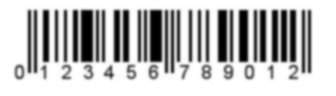
\includegraphics[width=0.35\textwidth]{img/EAN13/blurry_02_3.jpg}
  \caption{\surname{Gauß}'scher Weichzeichner mit 0,7 Pixeln und 3,0 Pixeln Radius}
  \label{fig:eanblurry}
\end{figure}

% rotierte
Das Problem von um $\alpha$ rotierten 1D Strichcodes ist, dass durch die Pixelbilder nie glatte Kanten entstehen können und somit keine sinnvolle Scanline gefunden werden kann oder sogar eine falsche erhalten wird~(Abbildung \ref{fig:eanrotate} Bild 3). Das zeigt sich vor allem bei Codes mit kürzeren Strichen, da dann weniger Platz für eine mögliche Scanline vorhanden ist, die zufällig die richtigen Entfernung erhalten hat. Daher kann auch der Beispielcode mit den längeren Strichen weiter gedreht werden, wie in Abbildung \ref{fig:eanrotate} zu sehen ist. Außerdem kann dort zusätzlich die Symmetrie der Erkennung von 1D Strichcodes bemerkt werden, da Codes auch bei $180^\circ \pm \alpha$ lesbar sind, wenn sie es bei $\alpha$ sind.

Bei rotierten Codes wirkt sich die unschärfe der Bilder nicht wesentlich auf die Erkennung aus, der Unschärfegrad ist genauso hoch möglich, wie ohne Drehung.
\begin{figure}[H]
  \centering
  \setlength{\fboxrule}{1pt}
  \fbox{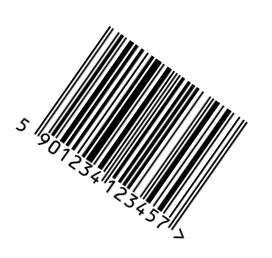
\includegraphics[height=4cm]{img/EAN13/rotate_01_35.jpg}}
  \fbox{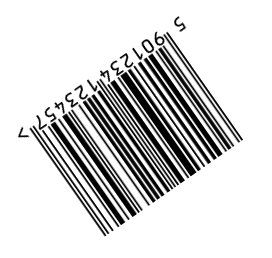
\includegraphics[height=4cm]{img/EAN13/rotate_01_145.jpg}}\\
  \fbox{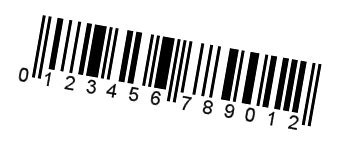
\includegraphics[height=1.9cm]{img/EAN13/rotate_02_10.jpg}}
  \fbox{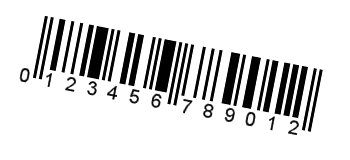
\includegraphics[height=1.9cm]{img/EAN13/rotate_02_11f.jpg}}
  \fbox{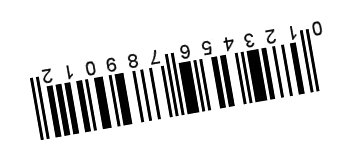
\includegraphics[height=1.9cm]{img/EAN13/rotate_02_170.jpg}}
  \fbox{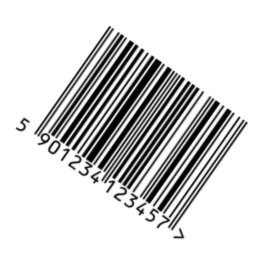
\includegraphics[height=4cm]{img/EAN13/blurryrotate_01_07_35.jpg}}
  \fbox{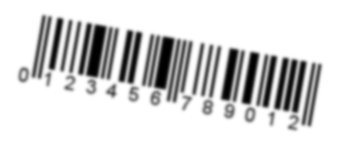
\includegraphics[height=1.9cm]{img/EAN13/blurryrotate_02_4_10.jpg}}
  \caption[EAN-13 Rotation]{Drehwinkel von 35$^\circ$, 145$^\circ$, 10$^\circ$~(falsch erkannt), 11$^\circ$, 170$^\circ$, 35$^\circ$~(unscharf) und 10$^\circ$~(unscharf)}
  \label{fig:eanrotate}
\end{figure}

% dunkle
Die Abdunkelung der Bilder hat keinen starken negativen Effekt auf die Erkennungsleistung, solange der Kontrast hoch genug bleibt. So können scharfe, unrotierte Strichcodes bis zu 90\% und selbst unscharfe, rotierte Bilder bis zu 80\% abgedunkelt werden~(Abbildung \ref{fig:eandark}).
\begin{figure}[H]
  \centering
  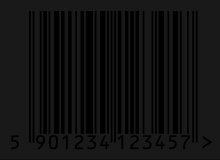
\includegraphics[width=0.30\textwidth]{img/EAN13/dark_01_90.jpg}
  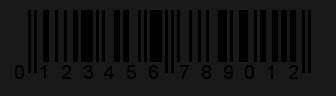
\includegraphics[width=0.35\textwidth]{img/EAN13/dark_02_90.jpg}
  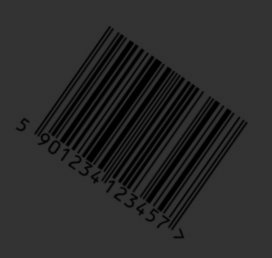
\includegraphics[width=0.35\textwidth]{img/EAN13/blurrydarkrotate_01_07_80_35.jpg}
  \caption{Bilder, die zu 90\%, 90\%und 80\% abgedunkelt sind.}
  \label{fig:eandark}
\end{figure}

% schatten
Da Schatten sich stark auf den Kontrast auswirken, können nur Strichcodes gelesen werden wo der Schatten nur um bis zu 20\% den Bildabschnitt verdunkelt und somit der Kontrast noch ausreichend hoch ist. In diesem Fall ist es auch ohne Bedeutung wie viel Fläche der Schatten überdeckt. Wenn allerdings eine lesbare Scanline zwischen den Schatten erhalten bleibt, dann ist der Code immer lesbar. Sich überlagernde Schatten, sind als jeweils einzelne Schatten anzusehen und können auch als solche bearbeitet werden.
\begin{figure}[H]
  \centering
  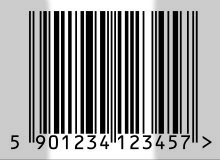
\includegraphics[height=3cm]{img/EAN13/shade_01_2x50+50.jpg}
  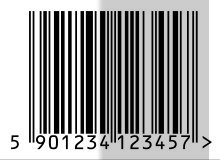
\includegraphics[height=3cm]{img/EAN13/shade_01_20+50.jpg}
  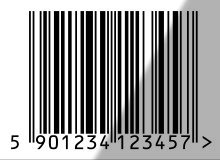
\includegraphics[height=3cm]{img/EAN13/shade_01_20+s30.jpg}
  \caption{Schatten die jeweils um 20\% abdunkeln}
  \label{fig:eanshade}
\end{figure}
